\chapter{Hashing Algorithms Based On The Merkle-Damg\r{a}rd  Construction}\label{chap:Merkle}

Nowadays, one-way hash functions are used in many cryptographic applications.\\
They are used for authentification, integrity checking, encryption and digital signatures (with public-key algorithms) and many security protocols. That's why, in order to guarantee their cryptographic robustness, they need to comply with various rules.

\section{Overview}

%Mathematical Purpose:
For many reasons, hash functions need to be one-way functions.
Ideally, each digest output by a hash function would match with single input message. This would guarantee the source message is the one we really expect, and that no different message could have been sent resulting in the same digest.

However in practice, such a property is not feasible, as hashing functions also guarantee a compression property, mapping an infinite starting set to a finite codomain.
Hash functions must therefore attempt, as far as possible, to avoid what are called collisions (two messages resulting in the same hash).

Moreover it is important that one cannot retrieve the original message, using only its hash.
If it were possible, the hash function would be useless, a malicious individual could compute a message resulting in a given hash, enabling him to send a different message than the one initially intended but using the same digest, and therefore the hash function would no longer guarantee a message's authenticity. For these reasons one-way hash functions need to respect various properties.

%Merkle-Damgard
To guarantee all these properties, it is often safest to ensure hashing functions respect established patterns to be fully efficient. Here, we will work on hash functions based on the Merkle-Damg\r{a}rd construction. %To built our digest, original message need to be expanded. 


\section{Cryptographic Requirements Of A Hash Function}~\label{sec:requirements}

One major requirement when building a hash functions is that it must be efficient, and therefore easy to compute. 
Other properties may also be required for cryptographic purposes.

\begin{defn}A collision between two different messages is a situation that occurs when two different messages $x \ne x'$ have the same hash value $H(x) = H(x')$.
\end{defn}
\begin{rem}
In so far as the input message of a hashing function can be of any length (in particular greater than the length of the output diggest), collisions are unavoidable.
\end{rem}
\begin{defn}
If y is such that $y = H(x)$, then x is a \emph{pre-image} for y (y being the \emph{hash} or \emph{digest}  of x).
\end{defn}

\begin{defn}~\label{def:sec_prop}
Hereafter are the three main properties a cryptographic hash function must fulfil:
\begin{itemize}
\item \textbf{Pre-image resistance}:  given $y$, it is hard to find a pre-image $x \in f^{-1}(H)$ such that $y = H(x)$.
\item \textbf{Second pre-image resistance}: given $x$, it is hard to find $x' \ne x$ such that $H(x) = H(x')$.
\item \textbf{Collision resistance}: it is hard to find two different messages $x' \ne x$ that have the same hash $H(x) = H(x')$.
\end{itemize}
\end{defn}

\begin{prop}Resistance to collisions implies second pre-image resistance which in turn implies pre-image resistance.
\end{prop}


\section{The Merkle-Damg\r{a}rd Construction}\label{sec:MerkleDamg}

The well known Merkle-Damg\r{a}rd construction describes how to construct a hash function based on a general compression function in an iterative structure. 

\begin{defn}A \emph{compression function} is a fixed input-size function which has an output length smaller than its input length: 
$$h:{\{0,1\}}^b ×{\{0,1\}}^n \rightarrow {\{0,1\}}^n$$
as depicted in figure~\ref{fig:compression}.
\end{defn}

\begin{figure}[H]
\centering
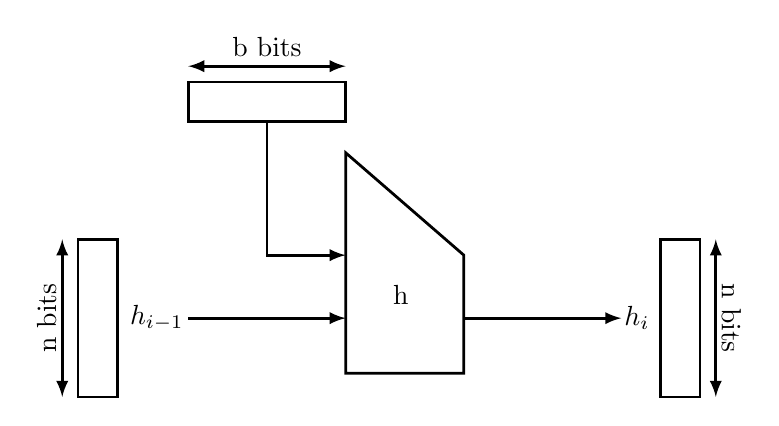
\begin{tikzpicture}

\draw[line width=1pt, name=h] (0,0) -- (0,2.8) -- (1.5,1.5) -- (1.5,0) -- cycle;
\node at(0.7,1){h};

\draw[line width=1pt] (-2,3.2) -- (0,3.2) -- (0,3.7) -- (-2,3.7) -- cycle;
\draw[<->, line width=1pt, >=latex] (-2,3.9) -- (0,3.9);
\node at (-1,4.15){b bits};
\draw[->, line width=1pt, >=latex] (-1,3.2) -- (-1,1.5) -- (0,1.5);


\draw[line width=1pt] (-3.4,-0.3) -- (-2.9,-0.3) -- (-2.9,1.7) -- (-3.4,1.7) -- cycle;
\node at (-2.4,0.7){$h_{i-1}$};
\draw[<->, line width=1pt, >=latex] (-3.6,-0.3) -- (-3.6,1.7);
\node[rotate=90] at (-3.8, 0.7){n bits};
\draw[->, line width=1pt, >=latex] (-2,0.7) -- (0,0.7);

\draw[line width=1pt] (4,-0.3) -- (4.5,-0.3) -- (4.5,1.7) -- (4,1.7) -- cycle;
\node at (3.7,0.7){$h_{i}$};
\draw[->, line width=1pt, >=latex] (1.5,0.7) -- (3.5,0.7);
\node[rotate=270] at (4.9, 0.7){n bits};
\draw[<->, line width=1pt, >=latex] (4.7,-0.3) -- (4.7,1.7);

\end{tikzpicture}
\caption{\label{fig:compression}Compression function.}
\end{figure}


Input values for the Merkle-Damg\r{a}rd construction are an n-bit IV (\emph{Initial Value}) and the arbitrary length input message. 
The IV is a fixed public value.

First the message $M$ is padded such that the entire padded message length be a multiple of the message block length b. The padded message is then separated into blocs of size exactly $b$ bits: $M_0,\ldots,M_{k-1}$.

The compression function h is then iterated according to the model depicted in figure~\ref{fig:constructionMD}.

\begin{figure}[ht]
\centering
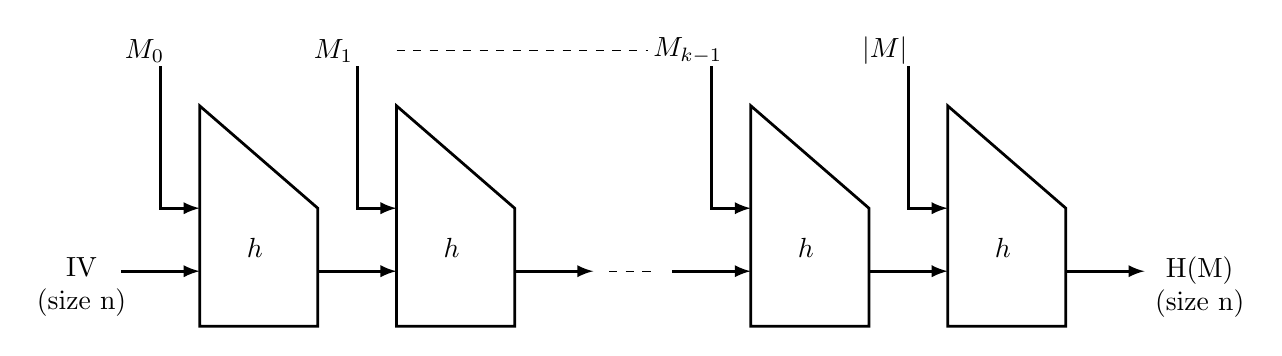
\begin{tikzpicture}

\node at (-0.7,3.5){$M_{0}$};
\draw[->, >=latex, line width=1pt] (-0.5,3.3) -- (-0.5,1.5) -- (0,1.5);
\node[align=center] at (-1.5,0.5){IV\\(size n)};
\draw[->, >=latex, line width=1pt] (-1,0.7) -- (0,0.7);
\draw[line width=1pt] (0,0) -- (0,2.8) -- (1.5,1.5) -- (1.5,0) -- cycle;
\node at(0.7,1){$h$};

\node at (1.7,3.5){$M_{1}$};
\draw[->, >=latex, line width=1pt] (2,3.3) -- (2,1.5) -- (2.5,1.5);
\draw[->, >=latex, line width=1pt] (1.5,0.7) -- (2.5,0.7);
\draw[line width=1pt] (2.5,0) -- (2.5,2.8) -- (4,1.5) -- (4,0) -- cycle;
\node at(3.2,1){$h$};
\draw[->, >=latex, line width=1pt] (4,0.7) -- (5,0.7);

\draw[dashed] (5.2,0.7) -- (5.8,0.7);
\draw[dashed] (2.5,3.5) -- (5.7,3.5);

\node at (6.2,3.5){$M_{k-1}$};
\draw[->, >=latex, line width=1pt] (6.5,3.3) -- (6.5,1.5) -- (7,1.5);
\draw[->, >=latex, line width=1pt] (6,0.7) -- (7,0.7);
\draw[line width=1pt] (7,0) -- (7,2.8) -- (8.5,1.5) -- (8.5,0) -- cycle;
\node at(7.7,1){$h$};

\node at (8.7,3.5){$|M|$};
\draw[->, >=latex, line width=1pt] (9,3.3) -- (9,1.5) -- (9.5,1.5);
\draw[->, >=latex, line width=1pt] (8.5,0.7) -- (9.5,0.7);
\draw[line width=1pt] (9.5,0) -- (9.5,2.8) -- (11,1.5) -- (11,0) -- cycle;
\node at(10.2,1){$h$};
\draw[->, >=latex, line width=1pt] (11,0.7) -- (12,0.7);
\node[align=center] at (12.7,0.5){H(M)\\(size n)};

\end{tikzpicture}
\caption{\label{fig:constructionMD}Merkle-Damg\r{a}rd construction.}
\end{figure}

A theorem demonstrated independently by Ralph Merkle and Ivan Damg\r{a}rd defines the theoretical properties of such a construction:
\begin{thm}
If the compression function $h$ is resistant to collision functions, then the resulting hash function $H$ is also.
\end{thm}


\begin{proof}
  We shall prove the theorem by contradiction:

  Let us assume that $H$ is not resistant to collisions, which means we can easily find $M$ and $M'$, such that $M \ne M'$ and $H(M)=H(M')$.
  Let us define $k$ and $l$ such that $k=\vert M\vert_b$ with $k \ge 1$ and $l=\vert M'\vert_b$ with $l \ge k$.
  We also define $y_0 = h^{k-1}(M)$ and $y_0' = h^{l-1}(M')$.\\
  Three cases may occur:
\begin{itemize}
\item Either $M_0,\ldots,M_{k-2}=M_0',\ldots,M_{k-2}'= u $. In which case $h(u \vert \vert M_{k-1})=h(u \vert \vert M_{k-1}',\ldots,M_{l-1}')$ we have found a collision for $h$.
\item Either $y_0 \ne y_0'$ and then since $h(y_0)=h(y_0')=H(M)=H(M')$ we have found a collision for $h$.
\item Either $y_0 = y_0'$ and $M_0,\ldots,M_{k-2} \ne M_0',\ldots,M_{k-2}'$. In which case we repeat the procedure with $y_i = h^{k-1-i}(M)$ and $y_i' = h^{l-1-i}(M')$ until $y_i \ne y_i'$.
\end{itemize}
\end{proof}


\paragraph{}

Consequently Merkle-Damg\r{a}rd is the most widespread construction used in calculating hashes.

Based on this construction, MD4 and MD5 formed an inspiration for other hash function designs that have followed over the years. They are all based on the Merkle-Damg\r{a}rd construction and have similar basic designs for their compression functions. The MD and SHA family of hash functions include (among others): MD4, MD5, SHA-0, SHA-1, the SHA2 family, RIPEMD \ldots




